\providecommand{\gddset}[2]{\expandafter\gdef\csname gddvalue@#1\endcsname{#2}}
\providecommand{\gddmissing}{\textcolor{blue}{\ensuremath{[\,\cdots\,]}}}
\providecommand{\gddresult}[1]{%
  \ifcsname gddvalue@#1\endcsname
    \expandafter\ifx\csname gddvalue@#1\endcsname\empty
      \gddmissing
    \else\csname gddvalue@#1\endcsname\fi
  \else\gddmissing\fi}
\providecommand{\gddci}[3]{\shortstack{\ensuremath{#1}\\[-1pt]{\scriptsize\ensuremath{[#2,#3]}}}}
\providecommand{\gddvaluesfile}{experiment_values.tex}
\InputIfFileExists{\gddvaluesfile}{}{}
\providecommand{\gddfigdir}{icde_sections/figures}
\providecommand{\gddimage}[3]{%
  \IfFileExists{\gddfigdir/#1.pdf}{%
    \includegraphics[width=\linewidth]{\gddfigdir/#1.pdf}%
  }{\IfFileExists{\gddfigdir/#1.png}{%
    \includegraphics[width=\linewidth]{\gddfigdir/#1.png}%
  }{%
    \fbox{\begin{minipage}[c][#2][c]{\dimexpr\linewidth-2\fboxsep-2\fboxrule\relax}
      \centering\small\sffamily #3\par\medskip
      \texttt{\detokenize{#1.pdf}}
    \end{minipage}}%
  }}%
}

% Reviewed experiment revision: RQ1--RQ4 and E1--E4 are retained.
% Enter dataset statistics, numerical results, and interpretation fields in icde_sections/experiment_values.tex.
% Figure filenames and cross-reference labels are defined in icde_sections/figures/.
% Empty result fields render as blue xxx; no empirical conclusion is prefilled.
\section{Experiments}\label{sec:gdd:en}
We evaluate PrivTDD's estimation accuracy, the contributions of its designs, sensitivity to the choice of regions, and the effect of sampling on TDD estimation error.
% We evaluate PrivTDD's estimation of the triangle-participation distribution through four research questions:
% \textbf{RQ1:} How accurately does PrivTDD estimate the distribution compared with existing methods?
% \textbf{RQ2:} How do structural modeling and learning correction strengths from private reports affect estimation?
% \textbf{RQ3:} How sensitive is PrivTDD to the choice of regions?
% \textbf{RQ4:} How does neighbor-pair sampling affect TDD estimation error on large networks?

\subsection{Experimental Setup}\label{sec:gdd:en:setup}

\noindent\textbf{Datasets.}
We use four real networks from SNAP and Network Repository~\cite{snapnets,rossi2015networkrepository}: the protein interaction network Bio-DMELA~\cite{singh2008alignment} with \gddresult{data.biodmela.n} nodes and \gddresult{data.biodmela.m} edges; 
the scientific collaboration network DBLP~\cite{yang2012communities} with \gddresult{data.dblp.n} nodes and \gddresult{data.dblp.m} edges; 
the social network Higgs social~\cite{dedomenico2013rumor} with \gddresult{data.higgs.n} nodes and \gddresult{data.higgs.m} edges; 
and Orkut~\cite{mislove2007measurement} with \gddresult{data.orkut.n} nodes and \gddresult{data.orkut.m} edges.
These networks cover different sizes, clustering levels, and TDDs.
We convert all inputs to simple undirected graphs, remove self-loops and duplicate edges, and retain all explicitly declared nodes and connected components; sizes refer to preprocessed graphs.

\noindent\textbf{Baselines.}
We compare PrivTDD with methods based on node-level counting and graph synthesis.
\textbf{TriTR-Hist} adapts TriTR~\cite{guo2026tritr}, 
a two-round triangle-counting estimator that Guo et al.\ identify as equivalent to TDP-VC~\cite{he2025robust}.
We adjust each node's estimate to count each incident triangle once, then clip, round, and bin the estimates.
%\textbf{TriTR-Hist}~\cite{guo2026tritr,he2025robust} converts TriTR's node triangle-participation estimates into a histogram, correcting counting multiplicities and applying clipping and rounding before binning~\cite{guo2026tritr}.
For LDPGraph~\cite{dong2026ldpgraph}, \textbf{LDPGraph-T} bins consistency-corrected node triangle-degree estimates, whereas \textbf{LDPGraph-S} recomputes the histogram on the final synthetic graph.
The outputs share private reports, isolating the effect of graph synthesis on TDD estimation.
Baselines follow their original parameter settings, adapted to the privacy-accounting convention used in this paper.

\begin{table*}[!t]
\centering
\caption{Estimation error on four networks across eight privacy budget settings}
\label{tab:gdd:e1:accuracy}
% One shade setting for all PrivTDD values. Larger numbers are lighter.
\newcommand*{\EOnePrivShade}{\cellcolor[gray]{0.90}}
\fontsize{8.5}{10}\selectfont
\setlength{\tabcolsep}{2.4pt}
\renewcommand{\arraystretch}{1.08}
\begin{tabularx}{\linewidth}{@{}lc *{12}{>{\raggedleft\arraybackslash}X}@{}}
\toprule
 &  & \multicolumn{3}{c}{PrivTDD (Ours)} & \multicolumn{3}{c}{TriTR-Hist} & \multicolumn{3}{c}{LDPGraph-T} & \multicolumn{3}{c}{LDPGraph-S} \\
\cmidrule(lr){3-5}\cmidrule(lr){6-8}\cmidrule(lr){9-11}\cmidrule(l){12-14}
Datasets & $\varepsilon$ & $10^3$\,MSE & EMD & $100$\,KS & $10^3$\,MSE & EMD & $100$\,KS & $10^3$\,MSE & EMD & $100$\,KS & $10^3$\,MSE & EMD & $100$\,KS \\
\midrule
\multirow{8}{*}{Bio-DMELA} & 0.5 & \EOnePrivShade 350.64 & \EOnePrivShade \textbf{20.39} & \EOnePrivShade \textbf{31.61} & 226.51 & 22145.74 & 49.98 & \textbf{221.81} & 965.06 & 45.60 & 615.10 & 739.05 & 57.95 \\
 & 1 & \EOnePrivShade \textbf{137.72} & \EOnePrivShade \textbf{5.05} & \EOnePrivShade \textbf{20.10} & 226.57 & 5406.54 & 49.70 & 215.78 & 175.16 & 41.51 & 505.46 & 149.62 & 50.06 \\
 & 1.5 & \EOnePrivShade \textbf{65.16} & \EOnePrivShade \textbf{2.89} & \EOnePrivShade \textbf{14.50} & 226.55 & 2453.85 & 49.38 & 205.95 & 68.61 & 37.96 & 447.99 & 61.65 & 46.75 \\
 & 2 & \EOnePrivShade \textbf{50.74} & \EOnePrivShade \textbf{2.03} & \EOnePrivShade \textbf{12.69} & 226.63 & 1425.10 & 49.02 & 193.47 & 36.39 & 35.05 & 409.87 & 33.96 & 44.45 \\
 & 2.5 & \EOnePrivShade \textbf{38.22} & \EOnePrivShade \textbf{1.58} & \EOnePrivShade \textbf{10.79} & 226.49 & 945.43 & 48.67 & 179.42 & 22.35 & 32.25 & 379.08 & 21.62 & 42.50 \\
 & 3 & \EOnePrivShade \textbf{21.24} & \EOnePrivShade \textbf{1.22} & \EOnePrivShade \textbf{8.05} & 226.44 & 681.66 & 48.34 & 164.62 & 15.19 & 30.03 & 347.25 & 15.30 & 40.47 \\
 & 3.5 & \EOnePrivShade \textbf{17.08} & \EOnePrivShade \textbf{1.00} & \EOnePrivShade \textbf{7.54} & 226.48 & 520.30 & 48.02 & 148.83 & 10.83 & 27.78 & 319.76 & 11.49 & 38.64 \\
 & 4 & \EOnePrivShade \textbf{12.46} & \EOnePrivShade \textbf{0.81} & \EOnePrivShade \textbf{6.42} & 226.38 & 413.88 & 47.71 & 133.93 & 8.31 & 25.64 & 293.49 & 9.28 & 36.87 \\
\midrule
\multirow{8}{*}{DBLP} & 0.5 & \EOnePrivShade \textbf{217.98} & \EOnePrivShade \textbf{9.33} & \EOnePrivShade \textbf{26.23} & 391.80 & 22090.15 & 49.08 & 386.00 & 919.83 & 35.96 & 294.10 & 887.25 & 36.21 \\
 & 1 & \EOnePrivShade \textbf{55.88} & \EOnePrivShade \textbf{4.62} & \EOnePrivShade \textbf{11.63} & 390.88 & 5382.79 & 47.97 & 369.61 & 157.12 & 34.66 & 331.00 & 153.39 & 32.99 \\
 & 1.5 & \EOnePrivShade \textbf{27.98} & \EOnePrivShade \textbf{3.59} & \EOnePrivShade \textbf{7.91} & 389.47 & 2437.97 & 46.97 & 347.42 & 57.16 & 34.15 & 318.82 & 56.63 & 33.14 \\
 & 2 & \EOnePrivShade \textbf{14.14} & \EOnePrivShade \textbf{2.65} & \EOnePrivShade \textbf{5.65} & 387.77 & 1412.67 & 46.00 & 323.21 & 28.24 & 33.37 & 298.46 & 28.51 & 32.68 \\
 & 2.5 & \EOnePrivShade \textbf{17.36} & \EOnePrivShade \textbf{2.09} & \EOnePrivShade \textbf{6.04} & 385.79 & 934.89 & 45.04 & 298.78 & 15.90 & 32.41 & 276.12 & 16.43 & 31.93 \\
 & 3 & \EOnePrivShade \textbf{12.40} & \EOnePrivShade \textbf{1.68} & \EOnePrivShade \textbf{5.75} & 383.63 & 672.32 & 44.12 & 275.68 & 10.02 & 31.30 & 255.05 & 10.88 & 31.01 \\
 & 3.5 & \EOnePrivShade \textbf{10.04} & \EOnePrivShade \textbf{1.40} & \EOnePrivShade \textbf{5.59} & 381.33 & 511.77 & 43.25 & 253.58 & 6.56 & 30.11 & 234.60 & 7.56 & 29.99 \\
 & 4 & \EOnePrivShade \textbf{10.01} & \EOnePrivShade \textbf{1.23} & \EOnePrivShade \textbf{5.69} & 378.92 & 405.98 & 42.44 & 234.47 & 4.75 & 28.91 & 216.86 & 5.75 & 28.92 \\
\midrule
\multirow{8}{*}{Higgs social} & 0.5 & \EOnePrivShade 24.55 & \EOnePrivShade \textbf{519.23} & \EOnePrivShade \textbf{14.42} & 301.41 & 26922.00 & 43.97 & 292.78 & 3845.87 & 37.15 & \textbf{7.29} & 4410.46 & 25.34 \\
 & 1 & \EOnePrivShade 29.00 & \EOnePrivShade \textbf{258.05} & \EOnePrivShade \textbf{17.44} & 292.42 & 6565.15 & 38.97 & 258.01 & 758.54 & 34.86 & \textbf{4.28} & 1969.99 & 18.80 \\
 & 1.5 & \EOnePrivShade 28.57 & \EOnePrivShade \textbf{130.81} & \EOnePrivShade 15.90 & 279.87 & 2904.04 & 36.22 & 212.93 & 261.19 & 31.63 & \textbf{3.32} & 1368.33 & \textbf{15.02} \\
 & 2 & \EOnePrivShade 27.28 & \EOnePrivShade \textbf{73.65} & \EOnePrivShade 13.03 & 265.88 & 1629.65 & 35.26 & 169.21 & 113.32 & 28.15 & \textbf{2.97} & 1092.75 & \textbf{12.71} \\
 & 2.5 & \EOnePrivShade 8.86 & \EOnePrivShade \textbf{45.52} & \EOnePrivShade 10.85 & 251.72 & 1042.36 & 34.25 & 132.34 & 57.61 & 24.86 & \textbf{2.72} & 1014.82 & \textbf{10.58} \\
 & 3 & \EOnePrivShade 4.79 & \EOnePrivShade \textbf{31.40} & \EOnePrivShade \textbf{9.10} & 237.95 & 725.90 & 33.24 & 102.75 & 33.06 & 21.86 & \textbf{2.59} & 984.85 & 9.24 \\
 & 3.5 & \EOnePrivShade 3.46 & \EOnePrivShade 23.32 & \EOnePrivShade \textbf{7.88} & 224.96 & 536.52 & 32.27 & 79.57 & \textbf{20.34} & 19.20 & \textbf{2.45} & 967.49 & 8.17 \\
 & 4 & \EOnePrivShade 2.66 & \EOnePrivShade 18.27 & \EOnePrivShade \textbf{6.98} & 213.04 & 414.59 & 31.35 & 62.90 & \textbf{14.00} & 17.03 & \textbf{2.40} & 962.87 & 7.49 \\
\midrule
\multirow{8}{*}{Orkut} & 0.5 & \EOnePrivShade \textbf{2.75} & \EOnePrivShade \textbf{182.69} & \EOnePrivShade \textbf{5.72} & 416.15 & 29051.16 & 45.25 & 402.88 & 5331.46 & 44.51 & 72.84 & 5215.75 & 27.31 \\
 & 1 & \EOnePrivShade \textbf{0.96} & \EOnePrivShade \textbf{116.53} & \EOnePrivShade \textbf{3.85} & 400.84 & 7186.61 & 44.40 & 344.76 & 1120.53 & 41.17 & 81.92 & 1123.67 & 26.80 \\
 & 1.5 & \EOnePrivShade \textbf{1.45} & \EOnePrivShade \textbf{66.66} & \EOnePrivShade \textbf{2.38} & 379.62 & 3201.31 & 43.20 & 272.57 & 418.09 & 36.60 & 86.11 & 446.54 & 25.74 \\
 & 2 & \EOnePrivShade \textbf{1.79} & \EOnePrivShade \textbf{35.58} & \EOnePrivShade \textbf{2.66} & 355.64 & 1803.13 & 41.80 & 205.70 & 197.35 & 31.78 & 90.89 & 234.14 & 24.60 \\
 & 2.5 & \EOnePrivShade \textbf{2.07} & \EOnePrivShade \textbf{21.15} & \EOnePrivShade \textbf{3.11} & 331.05 & 1154.47 & 40.31 & 152.26 & 107.46 & 27.33 & 81.16 & 148.65 & 21.97 \\
 & 3 & \EOnePrivShade \textbf{2.31} & \EOnePrivShade \textbf{15.20} & \EOnePrivShade \textbf{3.42} & 307.18 & 802.00 & 38.81 & 111.84 & 63.87 & 23.40 & 64.75 & 100.83 & 19.06 \\
 & 3.5 & \EOnePrivShade \textbf{2.37} & \EOnePrivShade \textbf{12.50} & \EOnePrivShade \textbf{3.59} & 284.79 & 589.83 & 37.35 & 82.25 & 40.34 & 20.05 & 48.92 & 76.07 & 16.31 \\
 & 4 & \EOnePrivShade \textbf{2.38} & \EOnePrivShade \textbf{11.00} & \EOnePrivShade \textbf{3.63} & 264.09 & 452.55 & 35.95 & 61.89 & 27.75 & 17.38 & 36.87 & 64.45 & 13.99 \\
\bottomrule
\end{tabularx}
\par\vspace{3pt}
\begin{minipage}{\linewidth}\fontsize{8}{9.3}\selectfont\raggedright Bold marks the lowest mean for each dataset, budget, and metric.
\end{minipage}
\end{table*}


\noindent\textbf{Metrics.}
We report mean squared error (MSE), earth mover's distance (EMD), and Kolmogorov--Smirnov distance (KS); lower is better.
Let $H$ and $\widehat H$ be the true and estimated node-count histograms, and let $F(t)=n^{-1}\sum_{u=0}^{t}H(u)$ be the true cumulative distribution, with $\widehat F$ defined analogously.
The metrics are
\begin{equation}
\begin{aligned}
&\mathrm{MSE}=\frac{\|\widehat H-H\|_2^2}{W_{\max}+1},\mathrm{EMD}=\|\widehat F-F\|_1,\\
&\mathrm{KS}=\|\widehat F-F\|_\infty,
\end{aligned}
\label{eq:gdd:en:metrics}
\end{equation}
where $W_{\max}=\binom{n-1}{2}$ and norms are evaluated on the integer triangle-degree domain $0,\ldots,W_{\max}$.
MSE compares node frequencies at each count; EMD accounts for both the probability mass displaced and its distance~\cite{rubner2000emd}; KS captures the largest cumulative-proportion discrepancy.
For PrivTDD, $\widehat H$ in these metrics is the released TDD in Eq.~\eqref{eq:pg-guard}.

\noindent\textbf{Implementation.}
We ran PrivTDD with \gddresult{hardware.software} on an \gddresult{hardware.processor} with \gddresult{hardware.memory.gib} GiB of memory.
For each network and privacy budget, we used the allocation in Eq.~\eqref{eq:pg-allocation} and set $\tau=1$.
By default, we use $K=\gddresult{settings.closure_components}$ closure-mixture components.
Following Section~\ref{sec:correction}, we define the body, transition, and tail regions using quantile levels $(\gddresult{settings.region_quantiles})$ of the base population distribution conditional on positive triangle degrees.
Complete parameters, baseline adaptations, and reproduction scripts are provided in the accompanying artifact.
%\footnote{Artifact: \gddresult{artifact.link}\label{fn:gdd:artifact}}
%todo in abstract+intro
% Budget optimality refers to the theoretical bound for the final safeguarded release.
% Budget optimality concerns the theoretical bound for the final release; the artifact supplies detailed implementation settings.
For E1 and E2, we scheduled \gddresult{runs.main.small_graphs} independent runs per setting on Bio-DMELA and DBLP and \gddresult{runs.main.large_graphs} on Higgs social and Orkut. We report means over completed runs and pointwise 95\% bootstrap confidence intervals.
Ablation variants share the private reports from each run.
For E4, we sampled candidate neighbor pairs after projection on Higgs social and Orkut at $\varepsilon=2$, using the same five seeds at each of the four sampling rates. Each run estimated the TDD of the full network.
% E4 fixes epsilon=2 on Higgs social and Orkut and samples projected candidate neighbor pairs. All four rates use the same five seeds and estimate the original graph TDD.
More details and results are available in the Supplementary Material. %give the full E1 intervals and paired E2 comparisons.
% E1/E2 plan 20 repetitions on each small graph and 10 on each large graph. Means and pointwise 95% bootstrap intervals use completed runs; E2 pairs the same private reports.

\subsection{Overall Estimation Accuracy (E1)}\label{sec:gdd:en:accuracy}
Table~\ref{tab:gdd:e1:accuracy} compares PrivTDD (shaded in gray) with TriTR-Hist, LDPGraph-T, and LDPGraph-S at eight total privacy budgets from $\varepsilon=0.5$ to $4$. %The means use 1,916 of 1,920 planned releases.
Across the four networks, PrivTDD had the lowest mean EMD in 30 of 32 network--budget settings, the lowest mean KS in 29, and the lowest mean MSE in 23.
Mean EMD decreased at every successive budget for PrivTDD on all four networks. MSE and KS varied less regularly. On Orkut, their minima occurred at $\varepsilon=1$ and $1.5$, respectively.
On DBLP at $\varepsilon=2$, the mean EMD of PrivTDD was 2.65 (95\% CI $[2.59,2.71]$), 90.6\% lower than the best baseline, LDPGraph-T (28.24).

PrivTDD ranked first on all three metrics at every budget on DBLP and Orkut. On Bio-DMELA, the single exception was MSE at $\varepsilon=0.5$, where LDPGraph-T had the lowest mean.
LDPGraph-S attained the lowest MSE at all eight budgets on Higgs social and the lowest KS at $\varepsilon\in\{1.5,2,2.5\}$. LDPGraph-T had the lowest EMD there at $\varepsilon\in\{3.5,4\}$.
Using only run indices completed by all four methods gave the same rankings in both settings with convergence failures.
To isolate the effect of synthesis, we compared the LDPGraph-T histogram with the histogram of the synthetic graph from the same private reports.
On the original metric scales, synthesis on Higgs social at $\varepsilon=2$ reduced MSE by 0.1662 and KS by 0.1544, while EMD rose by 979.4 (paired 95\% CI $[969.5,990.3]$).
On this network, synthesis reduced the bin-frequency error and the maximum CDF discrepancy but increased how far probability mass was displaced.


\subsection{Effects of the Core Designs (E2)}\label{sec:gdd:en:ablation}
PrivTDD, SCRec, and the three fixed-strength variants share the private reports, base fit, posterior reweighting, aggregation, and transport safeguard.
%Of 480 planned releases, 476 yielded all five outputs.
Two PrivTDD fits failed to converge on Higgs social at $\varepsilon=0.5$ and two on Orkut at $\varepsilon=4$, leaving eight matched runs in each setting.
% All five outputs share reports, base recovery, the final posterior update, aggregation, and transport safeguard. Of 480 planned conditions, 476 have complete five-method pairs; Higgs at 0.5 and Orkut at 4 each have two unconverged Full runs.

% Select one E2 figure layout.
% Four individual network plots share a single-column float, one legend and one caption.
\begin{figure}[tbhp]
\centering

\includegraphics[width=\columnwidth]{icde_sections/figures/gdd_ablation_key.pdf}\par
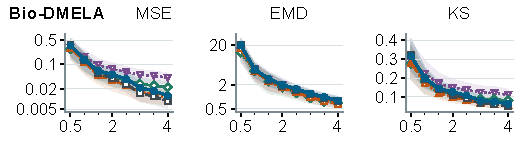
\includegraphics[width=\columnwidth]{icde_sections/figures/gdd_ablation_bio_dmela.pdf}\par
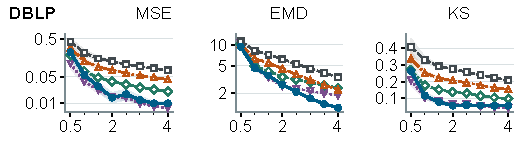
\includegraphics[width=\columnwidth]{icde_sections/figures/gdd_ablation_dblp.pdf}\par
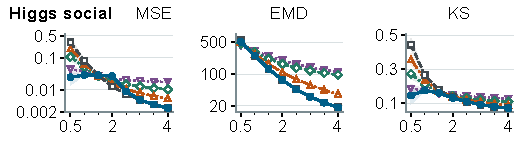
\includegraphics[width=\columnwidth]{icde_sections/figures/gdd_ablation_higgs.pdf}\par
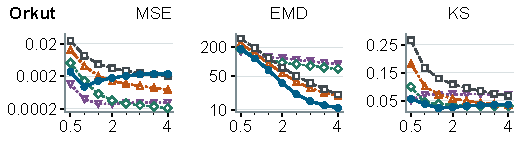
\includegraphics[width=\columnwidth]{icde_sections/figures/gdd_ablation_orkut.pdf}
\caption{Mean ablation errors versus privacy budget $\varepsilon$. Shading: pointwise 95\% bootstrap confidence intervals. MSE and EMD use log scales.}
\label{fig:gdd:en:ablation}
\end{figure}

% \input{icde_sections/figures/e2_wide.tex}  % Compact 3 x 4 double-column plot.
% \input{icde_sections/figures/e2_split.tex} % Two independently floating single-column blocks.

\noindent\textbf{Structural modeling and correction.}
SCRec (without structural correction) sets all seven correction strengths to zero.
On DBLP, enabling correction reduced mean MSE, EMD, and KS at all eight budgets (Fig.~\ref{fig:gdd:en:ablation}).
At $\varepsilon=2$, MSE fell from 0.1272 to 0.01414, EMD from 6.21 to 2.65 (mean paired reduction 3.56, 95\% CI $[3.49,3.63]$), and KS from 0.2755 to 0.0565.
On Orkut, correction reduced EMD and KS at every budget, but increased MSE at $\varepsilon=3.5$ and $4$.
On Bio-DMELA, mean EMD increased at every budget. On Higgs social at $\varepsilon=2$, correction increased MSE from 0.01272 to 0.02728 while reducing KS from 0.1334 to 0.1303.
%Separate reference ablations were available for 411 matched releases. 
On DBLP at $\varepsilon=2$, mean EMD was 2.65 with both references, 4.27 without the $\beta$ reference, and 5.83 without the geometric reference. On Bio-DMELA at the same budget, the corresponding means were 2.03, 2.02, and 1.90. Each of these comparisons used 20 matched runs.
% Removing either reference requires refitting. The independently verified reference-ablation coverage is 411 conditions; contributions vary by network.
 
\noindent\textbf{Learning correction strengths from reports.}
Fixed-0.25, Fixed-0.50, and Fixed-0.75 set each of the seven strengths to the specified value before projection onto the common feasible set in Eq.~\eqref{eq:joint_feasible_domain}.
PrivTDD learns these strengths from the reports using the same references, regions, and correction directions.
Across 32 network--budget settings, its mean error was lower than that of all three presets in 20 settings for EMD, 14 for KS, and seven for MSE.
On Orkut at $\varepsilon=2$, PrivTDD achieved an EMD of 35.58, compared with 57.66 for the best preset on this metric (Fixed-0.25).
On the same reports, Fixed-0.75 attained an MSE of 0.000287 versus 0.001788 for PrivTDD.
%On Bio-DMELA, a preset attained the lowest mean error for each metric at every budget.

\subsection{Sensitivity to the Choice of Regions (E3)}\label{sec:gdd:en:parameters}
% E3: sensitivity to the region partition.
We varied the body, transition, and tail regions used for report-driven distribution correction (Section~\ref{sec:correction}). On all four networks at $\varepsilon\in\{0.5,2\}$, we tested the quantile pairs $(0.80,0.90)$, $(0.90,0.95)$, and $(0.95,0.99)$. The middle pair is the default in E1 and E2. Each pair determines $b_1$ and $b_2$ from the base population distribution conditional on positive triangle degrees. The zero region stays fixed. 
% Vary body, transition, and tail regions using three quantile pairs; keep the zero region fixed. Reuse reports and base fits, refitting only correction strengths. Two Higgs base fits did not converge at epsilon=0.5.
The choice of regions had different effects across networks. Mean EMD varied little on Bio-DMELA and decreased at each step on DBLP at both budgets (Supplementary Material, Section~S3). Figure~\ref{fig:gdd:en:parameters} shows Higgs social and Orkut because raising both quantile levels from the lowest to the highest pair had opposite effects on these networks at $\varepsilon=0.5$. Mean EMD on Higgs social peaked at the default pair, then fell below its value at the lowest pair. On Orkut, it increased at both steps. At $\varepsilon=2$, the default gave the lowest mean EMD on Higgs social. The ordering on Orkut reversed, with mean EMD falling from 42.80 to 29.42 as the two levels increased, while both MSE and KS rose.
% Bio-DMELA EMD changes little; DBLP decreases at both budgets. Higgs and Orkut show opposite low-to-high changes at epsilon=0.5. Higgs is nonmonotone; at epsilon=2, Orkut EMD ordering reverses while MSE and KS rise.
\begin{figure}[htbp]
\centering
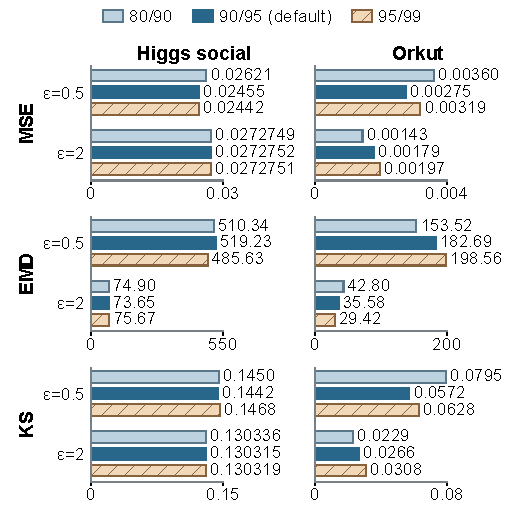
\includegraphics[width=\columnwidth]{icde_sections/figures/e3_sensitivity_means.pdf}
\caption{Sensitivity to the choice of regions on Higgs social and Orkut.}
\label{fig:gdd:en:parameters}
\end{figure}


Triangle-degree is more concentrated on Higgs social, where the top 1\% of nodes by triangle degree account for 47.6\% of the sum of triangle degrees, compared with 32.0\% on Orkut. To locate the errors at $\varepsilon=0.5$, we compared the estimates over the same percentile ranges of each network's true positive triangle-degree distribution. Moving from the lowest to the highest pair increased the EMD contribution between the 90th and 99th percentiles on both networks. On Higgs social, however, it reduced overestimation of the fraction of nodes above extreme triangle-degree thresholds. The EMD contribution above the 99.9th percentile fell in all eight paired runs, by 37.06 on average, and total mean EMD fell by 24.70. On Orkut, the same change worsened underestimation of the fraction of nodes above thresholds in the 90th--99th percentile range. The EMD contribution from this range alone rose by 43.85, close to the total increase of 45.04, and the contribution above the 99.9th percentile also rose.
% The top 1% of nodes carry a larger triangle-degree share on Higgs. Evaluation on fixed true-positive percentile ranges finds increasing 90th--99th percentile error on both networks. Reduced extreme-tail overestimation offsets other errors on Higgs; Orkut underestimation worsens. Truth is used only for evaluation.

\begin{table}[htbp]
\centering
\caption{TDD estimation error by neighbor-pair sampling rate at $\varepsilon=2$.}
% TDD estimation error at different neighbor-pair sampling rates.
\label{tab:gdd:e4:sampling}
\footnotesize
\setlength{\tabcolsep}{2pt}
\renewcommand{\arraystretch}{1.08}
\begin{tabular*}{\columnwidth}{@{\extracolsep{\fill}}lccc@{\hspace{8pt}}ccc@{}}
\toprule
\multirow{2}{*}{\shortstack[l]{Sampling rate}} & \multicolumn{3}{c}{Higgs social} & \multicolumn{3}{c}{Orkut} \\
\cmidrule(lr){2-4}\cmidrule(lr){5-7}
 & MSE & EMD & KS & MSE & EMD & KS \\
\midrule
0.01\% & 0.62058 & 582.89 & 0.5870 & 0.11288 & 945.85 & 0.3288 \\
0.1\% & 0.64318 & 537.15 & 0.5512 & 0.01495 & 2932.84 & 0.2963 \\
1\% & 0.29055 & 661.63 & 0.4008 & 0.13624 & 665.20 & 0.2277 \\
10\% & 0.02011 & 539.99 & 0.1342 & 0.00092 & 199.24 & 0.0453 \\
100\% (E1) & 0.02728 & 73.65 & 0.1303 & 0.00179 & 35.58 & 0.0266 \\
\bottomrule
\end{tabular*}
\end{table}

\subsection{Estimation Accuracy under Neighbor-Pair Sampling (E4)}\label{sec:gdd:en:cost}


On both networks, mean KS decreased at each successive sampling rate, and 10\% sampling gave the lowest mean MSE among the five settings (Table~\ref{tab:gdd:e4:sampling}).
On Higgs social, KS at 10\% sampling was close to that under full enumeration (0.1342 versus 0.1303), although mean EMD remained much higher (539.99 versus 73.65).
On Orkut, mean EMD was 199.24 at 10\% sampling and 35.58 under full enumeration.

